\section{并行直方图:原子操作和私有化简介}
到目前为止,我们提出的并行计算模式都允许将计算每个输出元素的任务专门分配给线程或由线程拥有。 
因此,这些模式符合所有者计算规则,其中每个线程都可以写入其指定的输出元素,而无需担心其他线程的干扰。 
本章介绍并行直方图计算模式,其中每个输出元素都可以由任何线程更新。 
因此,在更新输出元素时必须注意线程之间的协调,并避免任何可能破坏最终结果的干扰。 
在实践中,还有许多其他重要的并行计算模式,其中输出干扰无法轻易避免。 
因此,并行直方图算法提供了这些模式中发生的输出干扰的示例。 我们将首先检查使用原子操作序列化每个元素的更新的基线方法。 
这种基线方法简单但效率低下,常常导致执行速度令人失望。 
然后,我们将介绍一些广泛使用的优化技术,尤其是私有化,以显着提高执行速度,同时保持正确性。 
这些技术的成本和收益取决于底层硬件以及输入数据的特征。 
因此,对于开发人员来说,理解这些技术的关键思想并能够推理它们在不同情况下的适用性非常重要。

\subsection{背景}
直方图是数据集中数据值的计数或出现百分比的显示。 
在最常见的直方图形式中,值区间沿水平轴绘制,每个区间中的数据值计数表示为从水平轴上升的矩形或条形的高度。 
例如,直方图可用于显示短语“programming massively parallel processors. ”中字母表中字母的频率。 
为简单起见,我们假设输入短语全部为小写。 
通过检查,我们看到字母“a”有四个实例,字母“b”有零个实例,字母“c”有一个实例,依此类推。 
我们将每个值区间定义为四个字母的连续范围。 因此,第一个值区间是“a”到“d”,第二个值区间是“e”到“h”,依此类推。 
图 9.1 显示了一个直方图,根据我们对值区间的定义,显示了短语“编程大规模并行处理器”中字母的频率。

\begin{figure}[H]
	\centering
	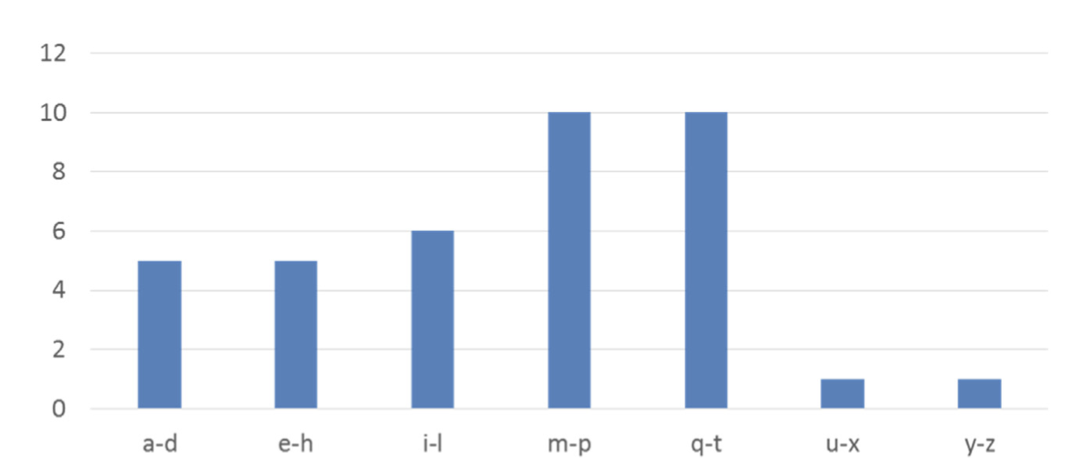
\includegraphics[width=0.9\textwidth]{figs/F9.1.png}
	\caption{\textit{"programming massively parallel processors." 的直方图表示}}
\end{figure}

直方图提供了有用的数据集摘要。 在我们的示例中,我们可以看到所表示的短语由大量集中在字母表中间间隔的字母组成,
而在后面的间隔中明显稀疏。 直方图的形状有时被称为数据集的特征,并提供一种快速方法来确定数据集中是否存在显着现象。 
例如,购买类别的直方图形状和信用卡帐户的位置可用于检测欺诈使用。 当直方图的形状明显偏离标准时,系统会提出潜在问题的标志。

许多应用领域依赖直方图来汇总数据集以进行数据分析。 计算机视觉就是这样的领域之一。 
不同类型的物体图像(例如人脸与汽车)的直方图往往呈现不同的形状。 例如,可以绘制图像或图像区域中像素发光值的直方图。 
这样的晴天天空直方图在发光光谱的高值区间中可能只有少量非常高的条形。 
通过将图像划分为子区域并分析这些子区域的直方图,人们可以快速识别图像中可能包含感兴趣对象的感兴趣的子区域。 
计算图像子区域直方图的过程是计算机视觉中特征提取的重要方法,其中特征指的是图像中感兴趣的模式。 
在实践中,每当需要分析大量数据以提取有趣的事件时,直方图就可能被用作基础计算。 信用卡欺诈检测和计算机视觉显然符合这一描述。 
具有此类需求的其他应用领域包括语音识别、网站购买推荐和科学数据分析,例如关联天体物理学中的天体运动。

\begin{figure}[H]
	\centering
	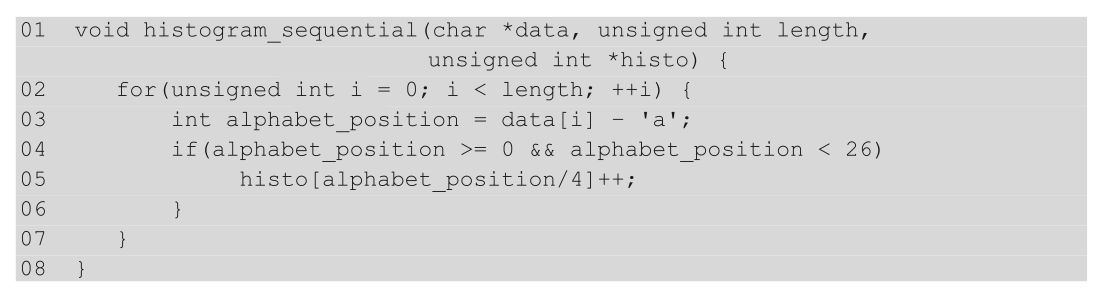
\includegraphics[width=0.9\textwidth]{figs/F9.2.png}
	\caption{\textit{一个简单的 C 函数,用于计算输入文本字符串的直方图。}}
\end{figure}

可以轻松地以顺序方式计算直方图。 图 9.2 显示了计算图 9.1 中定义的直方图的顺序函数。 
为简单起见,直方图函数需要仅识别小写字母。 
C 代码假设输入数据集采用 char 数组数据,并且直方图将生成到 int 数组 histo 中(第 01 行)。 
输入数据项的数量在函数参数长度中指定。 
for 循环(第 02-07 行)顺序遍历数组,识别已访问位置 data[i] 中字符的字母表索引,
将字母表索引保存到 Alphabet\_position 变量中,并递增与关联的 histo[alphabet\_position/4] 元素 那个间隔。 
字母索引的计算依赖于这样一个事实:输入字符串基于标准 ASCII 代码表示,
其中字母“a”到“z”根据其在字母表中的顺序被编码为连续值。

尽管人们可能不知道每个字母的确切编码值,但可以假设字母的编码值是“a”的编码值加上该字母与“a”之间的字母位置差。 
在输入中,每个字符都存储在其编码值中。 因此,表达式 data[i] - “a”(第 03 行)导出字母的字母表位置,
其中“a”的字母表位置为 0。如果位置值大于或等于 0 且小于 26,则 数据字符确实是一个小写字母(第 04 行)。 
请记住,我们定义了间隔,以便每个间隔包含四个字母。 因此,字母的间隔索引是其字母表位置值除以 4。
我们使用间隔索引来增加适当的 histo 数组元素(第 05 行)。

图 9.2 中的 C 代码非常简单且高效。 该算法的计算复杂度为 O(N),其中 N 是输入数据元素的数量。 
数据数组元素在 for 循环中按顺序访问,因此每当从系统 DRAM 获取数据时,CPU 缓存线都会得到很好的利用。 
histo 数组非常小,非常适合 CPU 的一级 (L1) 数据缓存,从而确保 histo 元素的快速更新。 
对于大多数现代 CPU,人们可以预期该代码的执行速度受到内存限制,即受到数据元素从 DRAM 进入 CPU 缓存的速率的限制。

\subsection{原子操作和基础直方图核函数}
\begin{figure}[H]
	\centering
	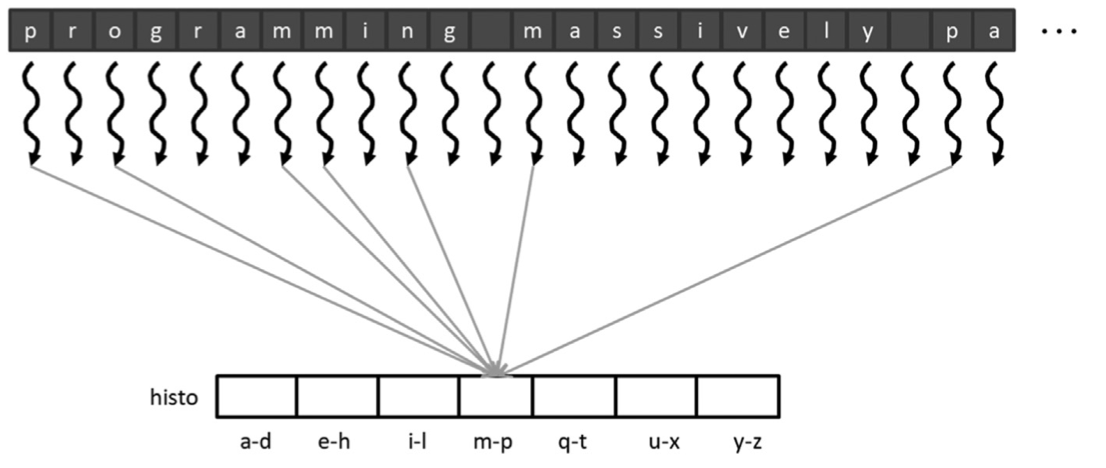
\includegraphics[width=0.9\textwidth]{figs/F9.3.png}
	\caption{\textit{直方图的基本并行化。}}
\end{figure}

并行化直方图计算的最直接方法是启动与数据元素一样多的线程,并让每个线程处理一个输入元素。 
每个线程读取其分配的输入元素并递增该字符的适当间隔计数器。 图 9.3 展示了这种并行化策略的一个例子。 
请注意,多个线程需要更新同一个计数器(m-p),这是一种冲突,称为输出干扰。 
程序员必须了解竞争条件和原子操作的概念,以便自信地处理并行代码中的此类输出干扰。

histo 数组中间隔计数器的增量是对内存位置的更新或读修改写操作。 
该操作包括读取内存位置(读)、将原始值加一(修改)以及将新值写回内存位置(写)。 读-修改-写是协调协作活动的常用操作。

例如,当我们向航空公司预订航班时,我们会调出座位图并查找可用座位(读取),选择要预订的座位(修改),
然后将座位图中的座位状态更改为不可用 (写)。 可能发生的不良情况如下:

• 两名乘客同时调出同一航班的座位图。

• 两位顾客选择相同的座位,例如9C。

• 两位客户均将座位9C 的状态更改为不可用。

排序结束后,两位顾客都认为自己的座位是 9C。 
可以想象,当他们登机时,发现其中一人不能坐在预定的座位上,会有一种不愉快的情况! 
不管你信不信,这种不愉快的情况在现实生活中时有发生,都是因为机票预订软件的缺陷造成的。

再比如,有些商店允许顾客无需排队等待服务。 他们要求每位顾客从其中一个售货亭获取一个号码。 
有一个显示屏显示接下来要服务的号码。 当服务代理有空时,代理会要求客户出示与号码匹配的票据,验证票据,
并将显示号码更新为下一个更大的号码。 理想情况下,所有顾客都将按照他们进入商店的顺序获得服务。 
不希望出现的结果是两个客户同时在两个自助服务终端登录,并且都收到具有相同号码的门票。 
当服务代理拨打该号码时,两位客户都希望自己是应该获得服务的人。

\begin{figure}[H]
	\centering
	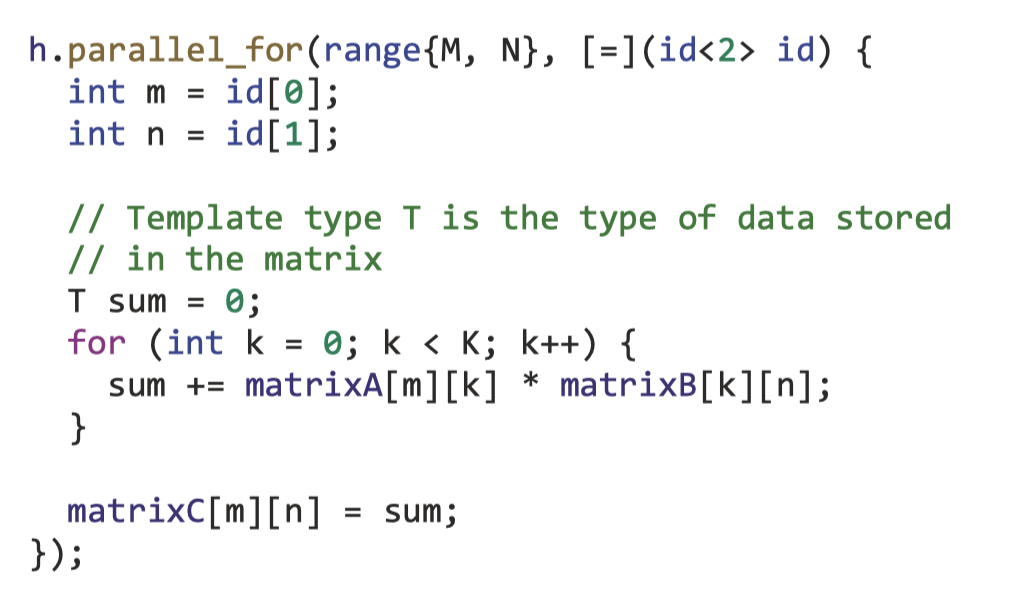
\includegraphics[width=0.9\textwidth]{figs/F9.4.png}
	\caption{\textit{更新 histo 数组元素时的竞争条件: (A) 一种可能的指令交错; (B) 另一种可能的指令交错。}}
\end{figure}

在这两个示例中,不良结果都是由称为“读取-修改-写入竞争条件”的现象引起的,
其中两个或多个同时更新操作的结果根据所涉及操作的相对时序而变化。 
\footnote{请注意,这与第 10 章“减少和最小化发散”中的读后写竞争条件类似,
但不相同,当时我们讨论了在每次Kogge-Stone 扫描内核迭代中对 XY 数组的读取和写入之间需要屏障同步。}
有些结果是正确的,有些结果是错误的。
图 9.4 说明了当两个线程尝试更新我们的文本直方图示例中的相同 histo 元素时的竞争条件。 
图 9.4 中的每一行显示了一段时间内的活动,时间从上到下进行。

图 9.4A 描述了这样一种场景,其中线程 1 在时间段 1 到 3 期间完成其读取-修改-写入序列的所有三个部分,
然后线程 2 在时间段 4 开始其序列。每个操作前面括号中的值 显示写入目标的值,假设 histo[x] 的值最初为 0。
在这种情况下,histo[x] 的值随后为 2,这正是人们所期望的。 也就是说,两个线程都成功增加了 histo[x]。 
元素值从0开始,运算完成后变为2。

在图 9.4B 中,两个线程的读取-修改-写入序列重叠。 请注意,线程 1 在时间段 4 将新值写入 histo[x]。
当线程 2 在时间段 3 读取 histo[x] 时,它的值仍然为 0。因此,它计算出的新值最终 写入 histo[x] 的是 1 而不是 2。
问题是线程 2 在线程 1 完成其更新之前过早读取 histo[x]。 最终结果是 histo[x] 之后的值为 1,这是不正确的。 
线程 1 的更新丢失。

\begin{figure}[H]
	\centering
	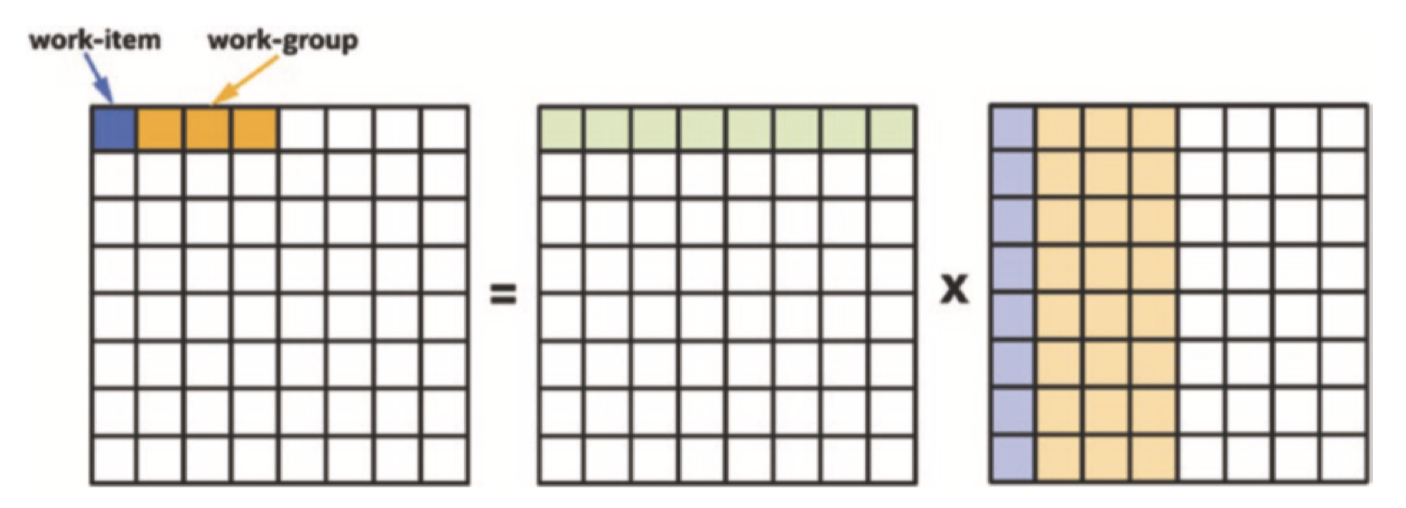
\includegraphics[width=0.9\textwidth]{figs/F9.5.png}
	\caption{\textit{线程 2 领先于线程 1 运行的竞争条件场景: (A) 一种可能的指令交错; (B) 另一种可能的指令交错。}}
\end{figure}

在并行执行期间,线程可以按相对于彼此的任何顺序运行。 在我们的示例中,线程 2 可以轻松地在线程 1 之前启动其更新序列。
图 9.5 显示了两个这样的场景。 在图 9.5A 中,线程 2 在线程 1 开始更新之前完成更新。 
在图 9.5B 中,线程 1 在线程 2 完成之前开始更新。 
显然,图 9.5A 中的序列会产生 histo[x] 的正确结果,但图 9.5B 中的序列会产生错误的结果。

histo[x] 的最终值根据所涉及操作的相对时间而变化,这一事实表明存在竞争条件。 
我们可以通过消除线程1和线程2的操作序列可能的交错来消除这种变化。也就是说,我们希望允许图 9.4A 和图 9.5A 所示的时序, 
同时消除图 9.4B 和 9.5B 中所示的可能性。 这可以通过使用原子操作来完成。

对内存位置的原子操作是在内存位置上执行读取-修改-写入序列的操作,其方式是对该位置的其他读取-修改-写入序列不能与其重叠。 
也就是说,操作的读取、修改和写入部分形成一个不可分割的单元,因此称为原子操作。 
实际上,原子操作是通过硬件支持来实现的,以将其他操作锁定到同一位置,直到当前操作完成。 
在我们的示例中,这种支持消除了图 1 和 2 中描述的可能性。 
9.4B 和 9.5B,因为在引导线程完成其更新序列之前,尾随线程无法开始其更新序列。

重要的是要记住,原子操作不会在线程之间强制执行任何特定的执行顺序。 在我们的示例中,图 1 和 2 中显示的两个顺序。 
9.4A 和 9.5A 是原子操作所允许的。 线程 1 可以在线程 2 之前或之后运行。
正在强制执行的规则是,如果两个线程在同一内存位置上执行原子操作,则尾随线程执行的原子操作无法启动,
直到线程 2 的原子操作完成为止。 主导线程完成。 这有效地序列化了在内存位置上执行的原子操作。

原子操作通常根据对内存位置执行的修改来命名。 在我们的文本直方图示例中,我们向内存位置添加一个值,因此原子操作称为原子添加。 
其他类型的原子操作包括减法、递增、递减、最小值、最大值、逻辑与和逻辑或。 
CUDA 内核可以通过函数调用对内存位置执行原子添加操作:

\begin{figure}[H]
	\centering
	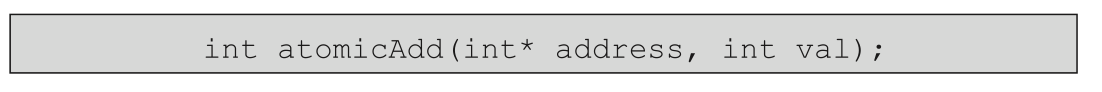
\includegraphics[width=0.9\textwidth]{figs/F9-a1.png}
\end{figure}

atomicAdd函数是一个内部函数(参见侧边栏“内部函数”),被编译成硬件原子操作指令。 
该指令读取全局或共享内存中地址参数指向的 32 位字,将 val 添加到旧内容,并将结果存储回内存中的同一地址。 
该函数返回该地址处的旧值。

\begin{figure}[H]
	\centering
	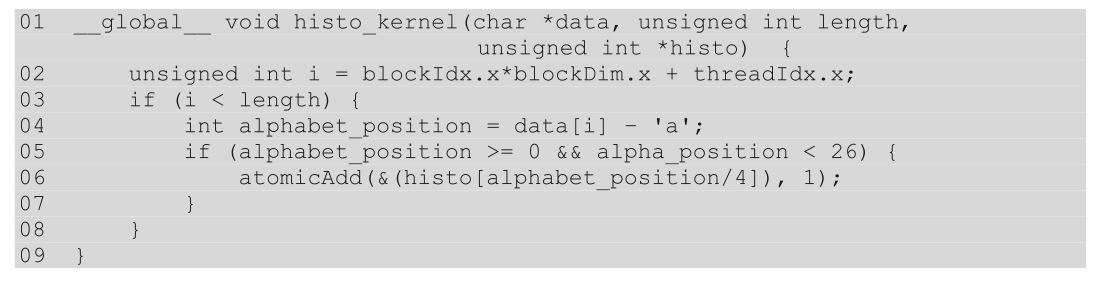
\includegraphics[width=0.9\textwidth]{figs/F9.6.png}
	\caption{\textit{用于计算直方图的 CUDA 内核。}}
\end{figure}

图 9.6 显示了执行并行直方图计算的 CUDA 内核。 该代码与图 9.2 中的顺序代码类似,但有两个关键区别。 
第一个区别是输入元素上的循环被线程索引计算(第 02 行)和边界检查(第 03 行)替换,以将线程分配给每个输入元素。 
第二个区别是图9.2中的增量表达式:

\begin{figure}[H]
	\centering
	
\includegraphics[width=0.9\textwidth]{figs/F9-a2.png}
\end{figure}

变成图 9.6 中的atomicAdd()函数调用(第06行)。 要更新的位置的地址 \&(histo[alphabet\_position/4]) 是第一个参数。
要添加到位置的值 1 是第二个参数。 这确保了不同线程对任何 histo 数组元素的任何同时更新都被正确序列化。

\begin{remark}[内部函数]
现代处理器通常提供特殊指令,这些指令要么执行关键功能(例如原子操作),要么显着增强性能(例如向量指令)。 
这些指令通常作为内在函数或简单地作为内在函数暴露给程序员。 从程序员的角度来看,这些都是库函数。 
然而,编译器以特殊的方式对待它们; 每个这样的调用都被翻译成相应的特殊指令。 
最终代码中通常没有函数调用,只有符合用户代码的特殊指令。 
所有主要的现代编译器,例如 GNU 编译器集合 (gcc)、Intel C 编译器和 Clang/LLVM C 编译器都支持内在函数。
\end{remark}

\subsection{原子操作的延迟和吞吐量}
图 9.6 的内核中使用的原子操作通过将任何同时更新序列化到某个位置来确保更新的正确性。 
众所周知,串行化大规模并行程序的任何部分都会大大增加执行时间并降低程序的执行速度。 
因此,此类串行操作占用尽可能少的执行时间非常重要。

正如我们在第 5 章“内存架构和数据局部性”中了解到的,DRAM 中数据的访问延迟可能需要数百个时钟周期。 
在第 4 章“计算架构和调度”中,我们了解到 GPU 使用零周期上下文切换来容忍此类延迟。 
在第 6 章“性能注意事项”中,我们了解到,只要有许多内存访问延迟可以相互重叠的线程,执行速度就会受到内存系统吞吐量的限制。 
因此,GPU 充分利用 DRAM 突发、存储体和通道来实现高内存访问吞吐量非常重要。

\begin{figure}[H]
	\centering
	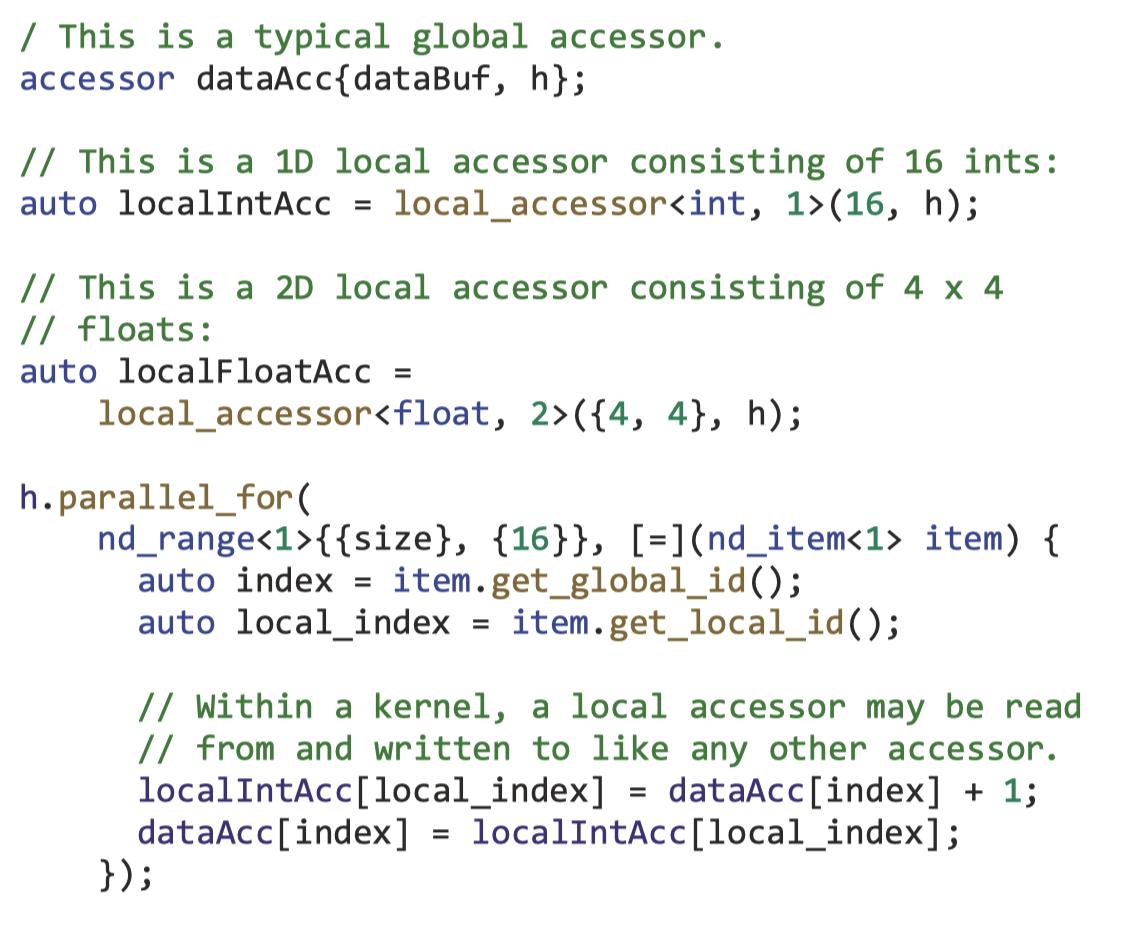
\includegraphics[width=0.9\textwidth]{figs/F9.7.png}
	\caption{\textit{原子操作的吞吐量由内存访问延迟决定。}}
\end{figure}

此时读者应该清楚,高内存访问吞吐量的关键是同时进行许多 DRAM 访问。 
不幸的是,当许多原子操作更新同一内存位置时,这种策略就会失效。 
在这种情况下,在引导线程的读取-修改-写入序列完成之前,尾随线程的读取-修改-写入序列无法启动。 
如图 9.7 所示,在同一内存位置执行原子操作时只能有一个正在进行。 
每个原子操作的持续时间大约是内存加载的延迟(原子操作时间的左侧部分)加上内存存储的延迟(原子操作时间的右侧部分)。 
每个读取-修改写入操作的这些时间部分的长度(通常为数百个时钟周期)定义了必须专用于服务每个原子操作的最小时间量,
并限制了吞吐量或可以执行原子操作的速率。

例如,假设存储器系统每通道具有 64 位(8 字节)双倍数据速率 DRAM 接口、八个通道、1 GHz 时钟频率
以及 200 个周期的典型访问延迟。 
内存系统的峰值访问吞吐量为 8(字节/传输)$\times$ 2(每个通道每个时钟的传输数)$\times$ 1 G(每秒时钟数)$\times$ 8(通道)= 128 GB/s。 
假设每个访问的数据是4字节,该系统的峰值访问吞吐量为每秒 32 G 数据元素。

然而,在特定内存位置执行原子操作时,可以实现的最高吞吐量是每 400 个周期执行一次原子操作
(200 个周期用于读取,200 个周期用于写入)。 
这意味着基于时间的吞吐量为 1/400 原子/时钟 $\times$ 1 G(时钟/秒)= 2.5 M 原子/秒。 
这大大低于大多数用户对 GPU 内存系统的期望。 此外,原子操作序列的长延迟可能会主导内核执行时间,
并可能显着降低内核的执行速度。

实际上,并非所有原子操作都将在单个内存位置上执行。 在我们的文本直方图示例中,直方图有七个间隔。 
如果输入字符均匀分布在字母表中,则原子操作将均匀分布在 histo 元素中。 
这会将吞吐量提高到每秒 7 $\times$ 2.5 M = 17.5 M 原子操作。 实际上,提升因子往往比直方图中的间隔数低得多,
因为字符在字母表中往往有偏差分布。 例如,在图 9.1 中,我们看到示例短语中的字符严重偏向 m-p 和 q-t 间隔。 
更新这些间隔的大量争用流量可能会将可实现的吞吐量降低到仅 (28/10) $\times$ 2.5 M = 7 M 左右。

提高原子操作吞吐量的一种方法是减少对竞争激烈的位置的访问延迟。 高速缓冲存储器是减少存储器访问延迟的主要工具。 
因此,现代 GPU 允许在最后一级缓存中执行原子操作,该缓存在所有流式多处理器 (SM) 之间共享。 
在原子操作过程中,如果在末级缓存中找到更新的变量,则在缓存中更新该变量。 
如果在最后一级缓存中找不到,则触发缓存未命中,并被带入缓存,并在那里进行更新。 
由于通过原子操作更新的变量往往会被许多线程大量访问,因此这些变量一旦从 DRAM 引入,往往会保留在缓存中。 
由于末级缓存的访问时间在数十个周期而不是数百个周期,因此原子操作的吞吐量比前几代GPU至少提高了一个数量级。 
这是大多数现代 GPU 支持末级缓存中原子操作的重要原因。

\subsection{私有化}
提高原子操作吞吐量的另一种方法是通过将流量引导远离竞争激烈的位置来减轻争用。 
这可以通过称为私有化的技术来实现,该技术通常用于解决并行计算中的严重输出干扰问题。 
这个想法是将高度竞争的输出数据结构复制到私有副本中,以便每个线程子集都可以更新其私有副本。 
好处是可以以更少的争用和更低的延迟来访问私有副本。 这些私有副本可以显着提高更新数据结构的吞吐量。 
缺点是计算完成后需要将私有副本合并到原始数据结构中。 人们必须在竞争程度和合并成本之间仔细权衡。 
因此,在大规模并行系统中,私有化通常是针对线程子集而不是单个线程进行的。

在我们的文本直方图示例中,我们可以创建多个私有直方图并指定线程子集来更新每个直方图。 
例如,我们可以创建两个私有副本,并使用偶数索引块来更新其中一个,使用奇数索引块来更新另一个。 
再举个例子,我们可以创建四个私有副本,并使用索引为 4n+i 形式的块来更新 $I = 0,\ldots , 3$ 的第 i 个私有版本
一种常见的方法是为每个线程块创建一个私有副本。 这种方法有多种优点,我们稍后会看到。

\begin{figure}[H]
	\centering
	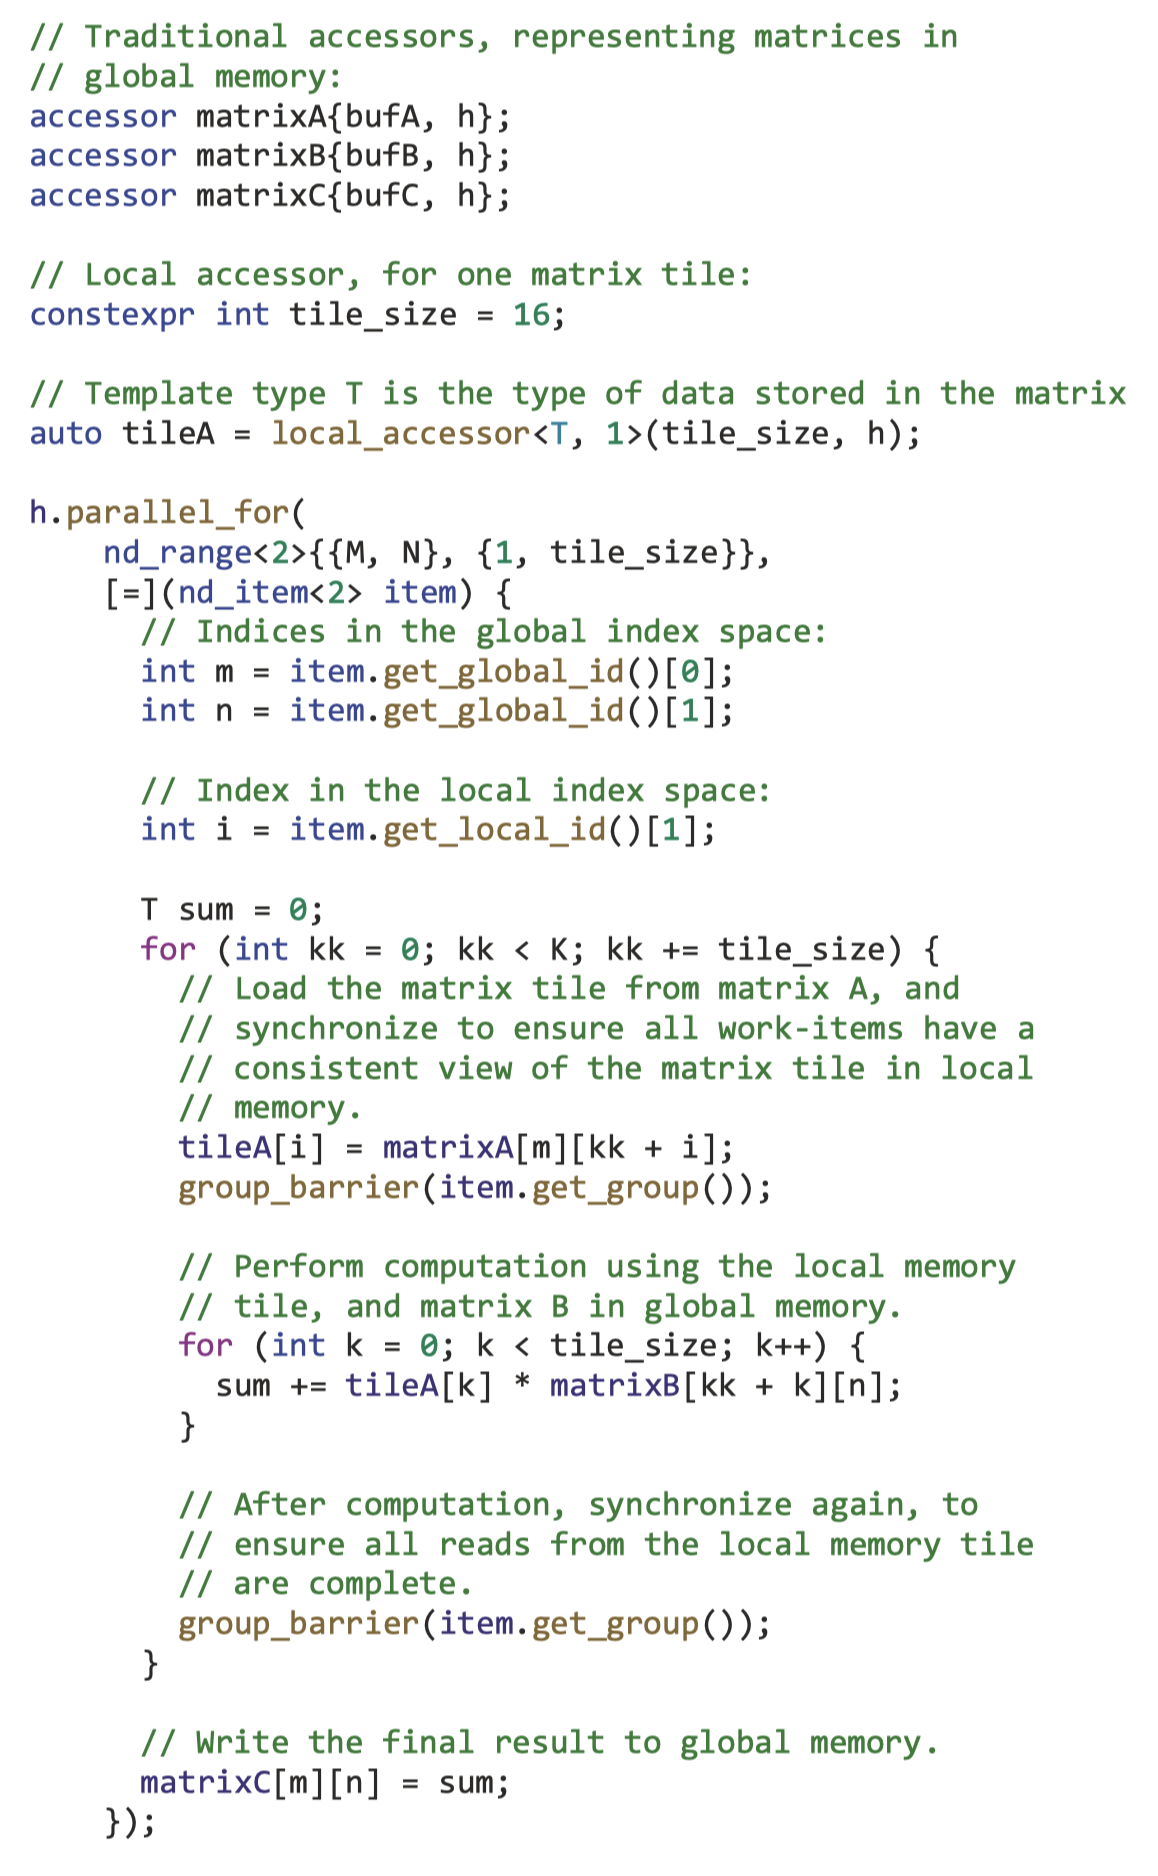
\includegraphics[width=0.9\textwidth]{figs/F9.8.png}
	\caption{\textit{直方图的私有副本减少了原子操作的争用。}}
\end{figure}

图 9.8 显示了如何将私有化应用于图 9.3 中的文本直方图示例。 
在此示例中,线程被组织成线程块,每个线程块由八个线程组成(实际上,线程块要大得多)。 
每个线程块都会收到它更新的直方图的私有副本。 
如图 9.8 所示,不会在更新同一直方图箱的所有线程之间发生争用,而是仅在同一块中的线程之间以及最后合并私有副本时才会遇到争用。

\begin{figure}[H]
	\centering
	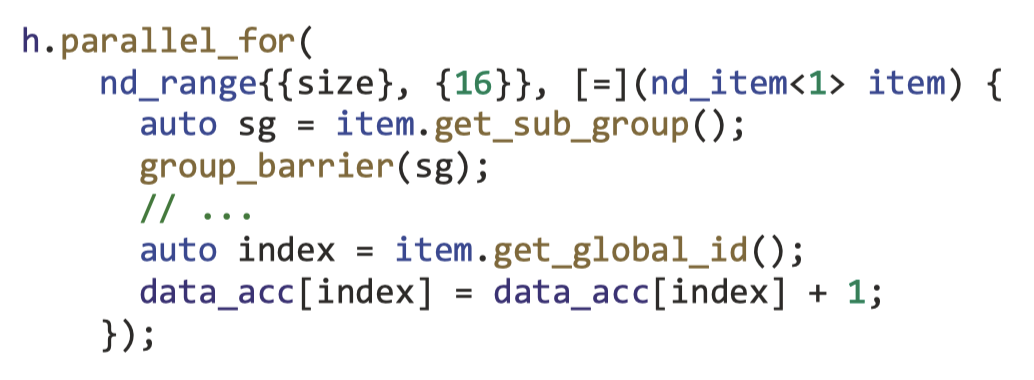
\includegraphics[width=0.9\textwidth]{figs/F9.9.png}
	\caption{\textit{线程块全局内存中具有私有版本的直方图内核。}}
\end{figure}

图 9.9 展示了一个简单的内核,它创建直方图的私有副本并将其关联到每个块。 在此方案中,最多 1024 个线程将处理直方图的副本。 
在此内核中,私有直方图位于全局内存中。 这些私有副本可能会缓存在 L2 缓存中,以减少延迟并提高吞吐量。

图 9.9 中的内核的第一部分(第 02-08 行)与图 9.6 中的内核类似,但有一个关键区别。 
图 9.9 中的内核假设主机代码将为 histo 数组分配足够的设备内存来保存直方图的所有私有副本,
总计为 gridDim.x * NUM\_BINS * 4 字节。 这反映在第 06 行,其中每个线程添加了 blockIdx 的偏移量。 
对直方图元素(直方图的 bin)执行原子添加时,将 x * NUM\_BINS 添加到索引。 
此偏移量将位置移动到线程所属块的私有副本。 在这种情况下,争用程度会降低一个因子,该因子大约是所有 SM 上的活动块的数量。 
减少争用的效果可以使内核的更新吞吐量提高几个数量级。

在执行结束时,每个线程块都会将私有副本中的值提交到块 0 生成的版本中(第 09-17 行)。 
也就是说,我们将块 0 的私有副本提升为公共副本,该副本将保存所有块的总结果。 
块中的线程首先等待彼此完成更新私有副本(第 10 行)。 接下来,线程迭代私有直方图箱(第 11 行),
每个线程负责提交一个或多个私有箱。 循环用于容纳任意数量的容器。 
每个线程读取它负责的私有 bin 的值(第 13 行)并检查该 bin 是否非零(第 13 行)。 
如果是,则线程通过原子地将值添加到块 0 的副本(第 14 行)来提交该值。 
请注意,加法需要以原子方式执行,因为来自多个块的线程可以同时在同一位置执行加法。 
因此,在内核执行结束时,最终的直方图将位于 histo 数组的前 NUM\_BINS 个元素中。 
由于在内核执行的这一阶段,每个块中只有一个线程将更新任何给定的 histo 数组元素,因此每个位置的争用级别非常适中。

在每个线程块的基础上创建直方图的私有副本的好处之一是线程可以在提交之前使用 \_\_syncthreads() 相互等待。 
如果私有副本被多个块访问,我们将需要调用另一个内核来合并私有副本或使用其他复杂的技术。 
在每个线程块的基础上创建直方图的私有副本的另一个好处是,如果直方图中的 bin 数量足够小,
则可以在共享内存中声明直方图的私有副本。 如果私有副本被多个块访问,则无法使用共享内存,因为块不具有彼此共享内存的可见性。

回想一下,延迟的任何减少都会直接转化为同一内存位置上原子操作的吞吐量的提高。 
通过将数据放入共享内存中可以显着减少访问内存的延迟。 共享内存是每个 SM 私有的,并且具有非常短的访问延迟(几个周期)。 
这种延迟的减少直接转化为原子操作吞吐量的增加。

\begin{figure}[H]
	\centering
	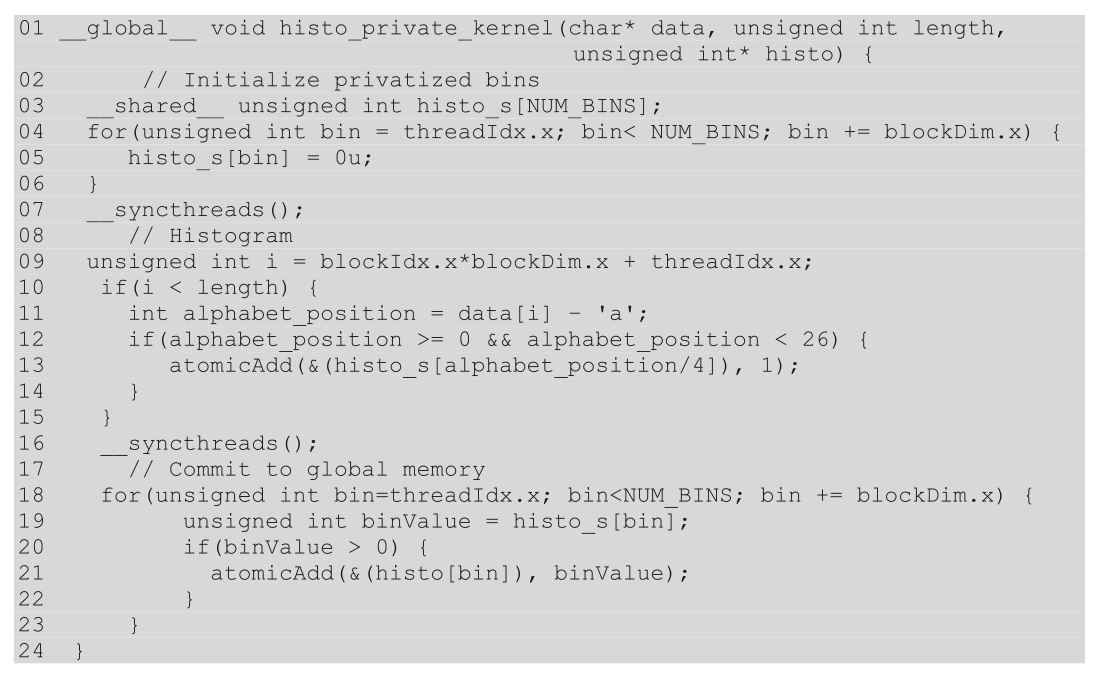
\includegraphics[width=0.9\textwidth]{figs/F9.10.png}
	\caption{\textit{使用共享内存的私有化文本直方图内核。}}
\end{figure}

图 9.10 显示了一个私有化直方图内核,它将私有副本存储在共享内存而不是全局内存中。 
与图 9.9 中的内核代码的主要区别在于,直方图的私有副本分配在 histo\_s 数组的共享内存中,
并由块的线程并行初始化为 0(第 02-06 行)。 
屏障同步(第 07 行)确保私有直方图的所有 bin 在任何线程开始更新它们之前都已正确初始化。 
其余代码与图 9.9 中的代码相同,只是第一个原子操作是对共享内存数组 histo\_s 的元素执行的(第 13 行),
并且稍后从那里读取私有 bin 值(第 19 行)。

\subsection{粗化}
我们已经看到,私有化可以有效减少原子操作的争用,并且将私有化直方图存储在共享内存中可以减少每个原子操作的延迟。 
然而,私有化的开销是需要将私有副本提交给公共副本。 每个线程块执行一次此提交操作。 因此,我们使用的线程块越多,开销就越大。 
当线程块并行执行时,这种开销通常是值得的。 
但是,如果启动的线程块的数量超过了硬件可以同时执行的数量,则硬件调度会将这些线程块串行化。 
在这种情况下,就会产生不必要的私有化开销。

我们可以通过线程粗化来减少私有化的开销。 
换句话说,我们可以通过减少块的数量并让每个线程处理多个输入元素来减少提交给公共副本的私有副本的数量。 
在本节中,我们将研究将多个输入元素分配给线程的两种策略:连续分区和交错分区。

\begin{figure}[H]
	\centering
	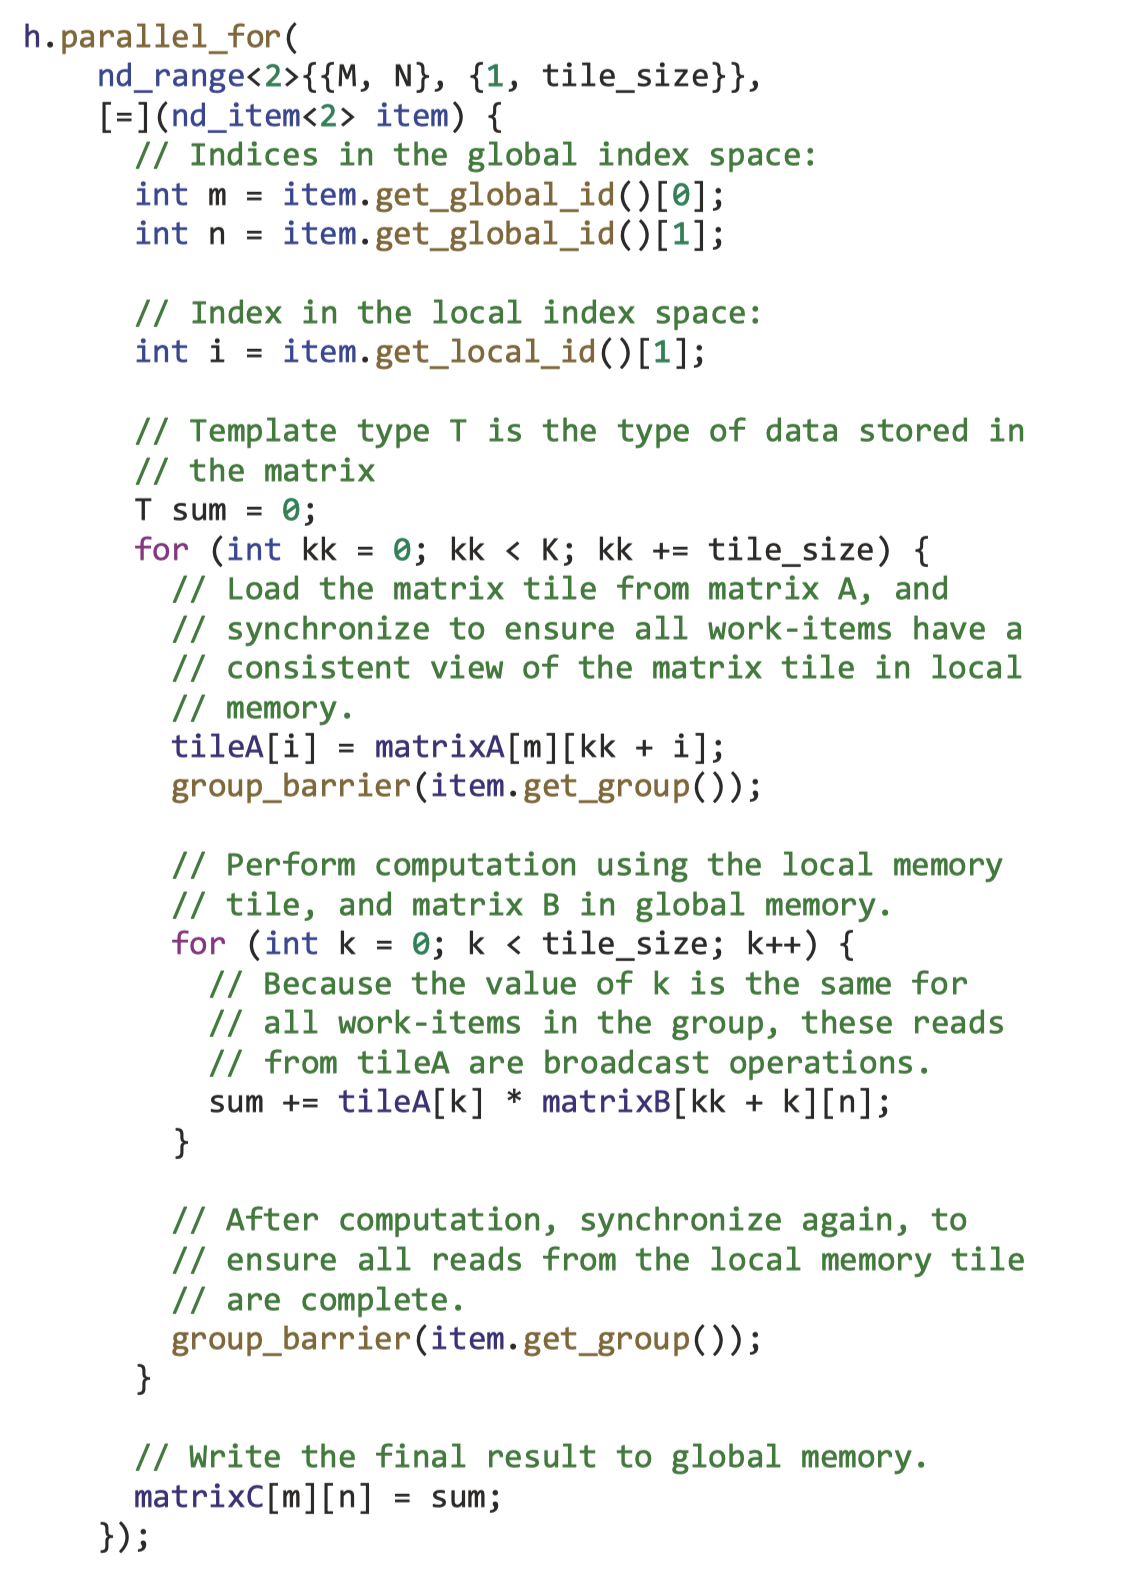
\includegraphics[width=0.9\textwidth]{figs/F9.11.png}
	\caption{\textit{输入元素的连续分区。}}
\end{figure}

\begin{figure}[H]
	\centering
	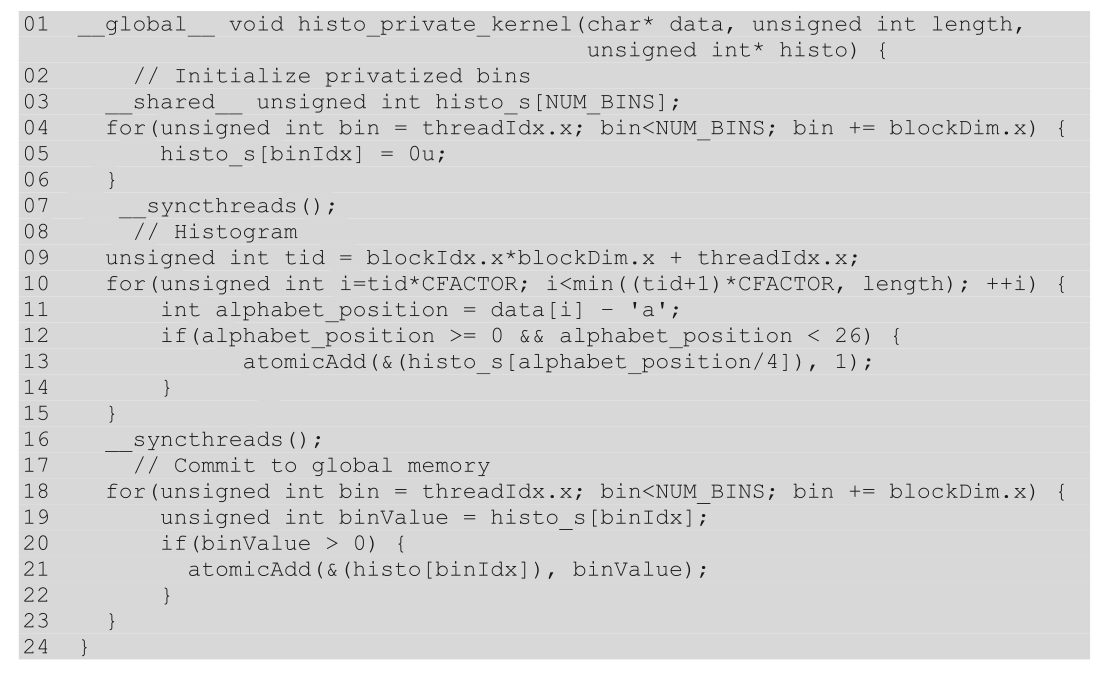
\includegraphics[width=0.9\textwidth]{figs/F9.12.png}
	\caption{\textit{使用连续分区进行粗化的直方图内核。}}
\end{figure}

图 9.11 显示了连续分区策略的示例。 输入被划分为连续的段,每个段被分配给一个线程。 
图 9.12 显示了使用连续分区策略应用粗化的直方图内核。 与图 9.10 的区别在于第 09-10 行。 
在图9.10中,输入元素索引i对应于全局线程索引,因此每个线程接收一个输入元素。 
在图 9.11 中,输入元素索引 i 是从 tid * CFACTOR 迭代到 (tid + 1) * CFACTOR 的循环的索引,其中 CFACTOR 是粗化因子。 
因此,每个线程都采用 CFACTOR 元素的连续段。 循环边界中的min操作确保末尾的线程不会读取越界。

将数据划分为连续的段在概念上简单且直观。 
在并行执行通常涉及少量线程的 CPU 上,连续分区通常是性能最佳的策略,因为每个线程的顺序访问模式充分利用了缓存行。 
由于每个CPU缓存通常只支持少量线程,因此不同线程对缓存的使用几乎没有干扰。 
高速缓存行中的数据一旦被线程引入,就可以保留以供后续访问。

相比之下,GPU 上的连续分区会导致内存访问模式不理想。 
正如我们在第 5 章“内存体系结构和数据局部性”中了解到的,SM 中大量同时活动的线程通常会对缓存造成很大的干扰,
以至于无法期望单个线程的所有顺序访问都将数据保留在缓存中 。 
相反,我们需要确保 warp 中的线程访问连续的位置以启用内存合并。 这一观察激发了交错分区。

\begin{figure}[H]
	\centering
	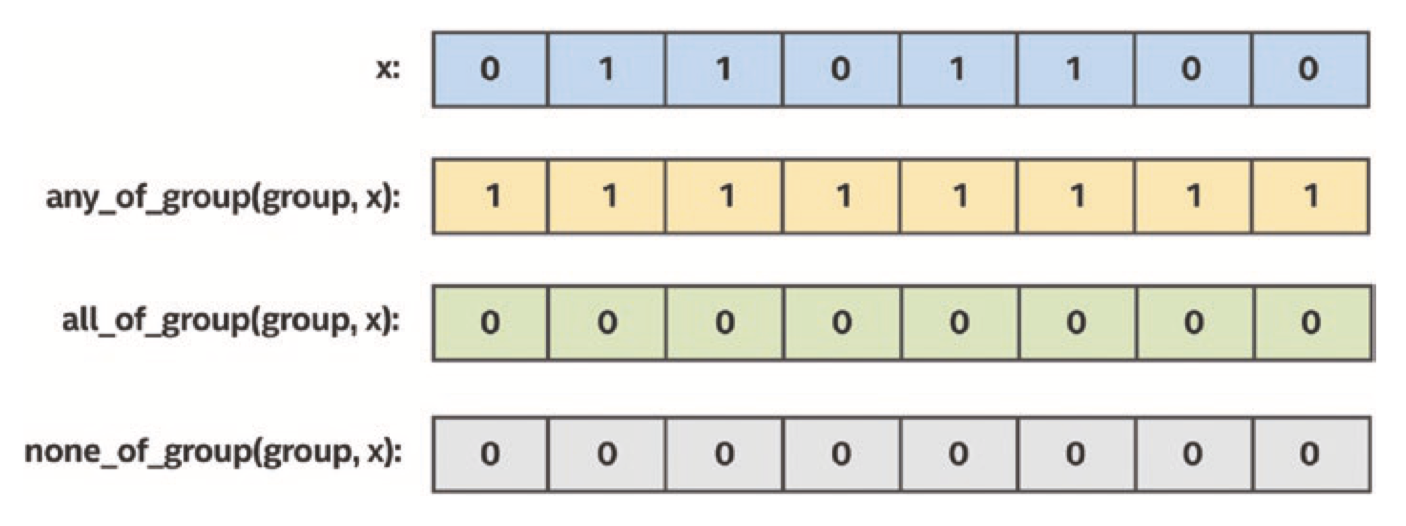
\includegraphics[width=0.9\textwidth]{figs/F9.13.png}
	\caption{\textit{输入元素的交错分区。}}
\end{figure}

图 9.13 显示了交错分区策略的示例。 在第一次迭代期间,八个线程访问字符 0 到 7(“programm”)。 
通过内存合并,只需一次 DRAM 访问即可获取所有元素。 在第二次迭代期间,四个线程在一次合并的内存访问中访问字符“ingmass”。 
应该清楚为什么这被称为交错分区:不同线程要处理的分区是相互交错的。 显然,这是一个玩具示例,实际上,会有更多线程。 
还有更微妙的性能考虑因素。 例如,每个线程应在每次迭代中处理四个字符(一个 32 位字),以充分利用缓存和 SM 之间的互连带宽。

\begin{figure}[H]
	\centering
	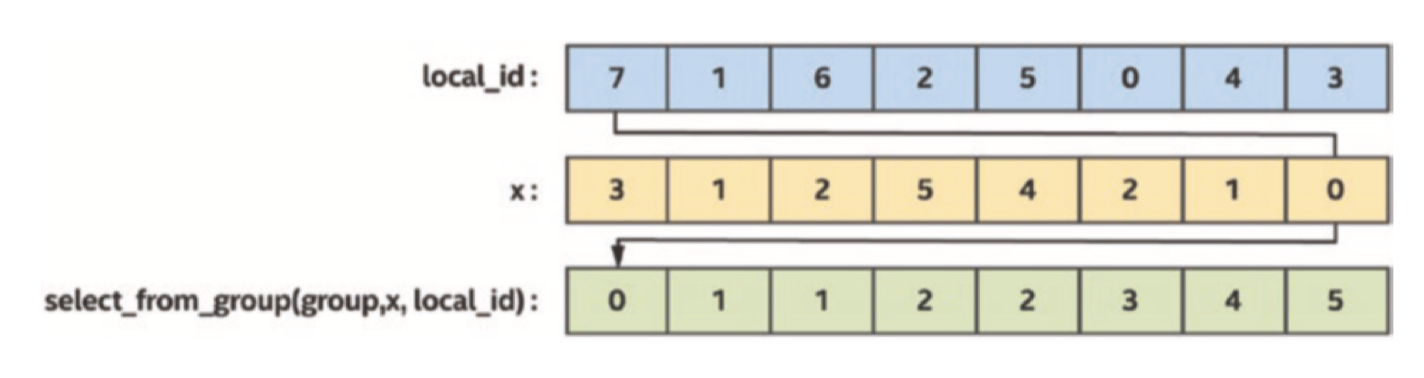
\includegraphics[width=0.9\textwidth]{figs/F9.14.png}
	\caption{\textit{使用交错分区进行粗化的直方图内核。}}
\end{figure}

图 9.14 显示了使用交错分区策略进行粗化的直方图内核。 与图 9.10 和 9.12 的区别再次位于第 09-10 行。 
在循环的第一次迭代中,每个线程使用其全局线程索引访问数据数组:线程 0 访问元素 0,线程 1 访问元素 1,线程 2 访问元素 2,
依此类推。 因此,所有线程联合处理输入的第一个 blockDim.x * gridDim.x 元素。 
在第二次迭代中,所有线程将 blockDim.x * gridDim.x 添加到其索引中,并联合处理 blockDim.x * gridDim.x 元素的下一部分。

当线程的索引超出输入缓冲区的有效范围(其私有 i 变量值大于或等于 length)时,该线程已完成其分区的处理并将退出循环。 
由于缓冲区的大小可能不是线程总数的倍数,因此某些线程可能不参与最后一部分的处理。 
因此,某些线程将比其他线程少执行一次循环迭代。

\subsection{聚集}
一些数据集在局部区域大量集中相同的数据值。 例如,在天空图片中,可能存在大块具有相同值的像素。 
如此高度集中的相同值会导致严重争用并降低并行直方图计算的吞吐量。

对于此类数据集,一个简单而有效的优化是,如果每个线程正在更新直方图的相同元素,则将连续更新聚合为单个更新(Merrill,2015)。 
这种聚合减少了对高度竞争的直方图元素的原子操作的数量,从而提高了计算的有效吞吐量。

\begin{figure}[H]
	\centering
	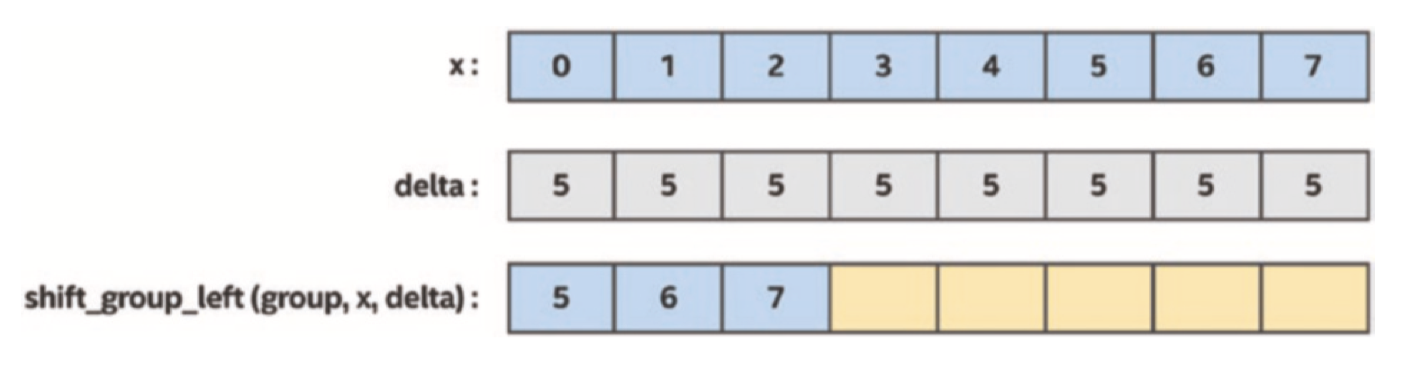
\includegraphics[width=0.9\textwidth]{figs/F9.15.png}
	\caption{\textit{聚合文本直方图内核。}}
\end{figure}

图 9.15 显示了聚合文本直方图内核。 与图 9.14 中的内核相比,关键变化如下:每个线程声明一个附加的累加器变量(第 09 行),
用于跟踪迄今为止聚合的更新数量,以及一个 prevBinIdx 变量(第 10 行),用于跟踪索引 最后遇到且正在聚合的直方图 bin。 
每个线程将累加器变量初始化为零,表示最初尚未聚合任何更新,并将 prevBinIdx 初始化为 21,以便没有字母输入与其匹配。

当找到字母表数据时,线程将要更新的直方图元素的索引与正在聚合的直方图元素的索引进行比较(第 16 行)。 
如果索引相同,则线程只需递增累加器(第 17 行),将聚合更新的连续次数延长 1。 
如果索引不同,则直方图元素的聚合更新的连续性已结束。 
该线程使用原子操作将累加器值添加到索引由 prevBinIdx 跟踪的直方图元素(第 19-21 行)。 这有效地清除了先前聚合更新的总贡献。

使用这种方案,更新总是至少落后一个元素。 在没有连续的极端情况下,所有更新将始终落后一个元素。 
这就是为什么线程完成扫描所有输入元素并退出循环后,线程需要检查是否需要刷新累加器值(第27行)。 
如果是,则累加器值将刷新到右侧的 histo\_s 元素(第 28 行)。

一项重要的观察结果是聚合内核需要更多语句和变量。 因此,如果争用率较低,则聚合内核的执行速度可能低于简单内核。 
然而,如果数据分布导致原子操作执行中的严重争用,聚合可能会导致显着更高的速度。 添加的 if 语句可能会出现控制发散。 
然而,如果没有争用或严重争用,则控制发散很小,因为线程要么全部刷新累加器值,要么全部处于连续状态。 
在某些线程处于连续状态而某些线程将刷新其累加器值的情况下,控制发散可能会通过减少争用来补偿。

\subsection{总结}
计算直方图对于分析大型数据集非常重要。 它还代表了一类重要的并行计算模式,其中每个线程的输出位置是数据相关的,
这使得应用所有者计算规则不可行。 因此,它是引入读-修改-写竞争条件概念和原子操作实际使用的自然工具,
以确保对同一内存位置的并发读-修改-写操作的完整性。

不幸的是,正如我们在本章中所解释的,原子操作的吞吐量比简单的内存读取或写入操作低得多,
因为它们的吞吐量大约是内存延迟两倍的倒数。 因此,在存在严重争用的情况下,直方图计算的计算吞吐量可能低得惊人。 
私有化作为一种重要的优化技术被引入,它可以系统地减少争用,并可以进一步启用共享内存的使用,从而支持低延迟和高吞吐量。 
事实上,支持块中线程之间的快速原子操作是共享内存的一个重要用例。 
还应用粗化来减少需要合并的私有副本的数量,并比较了使用连续分区和交错分区的不同粗化策略。 
最后,对于导致严重争用的数据集,聚合还可以显着提高执行速度。
